\documentclass[12pt]{article}
\usepackage[utf8]{inputenc}
\usepackage{mathtools}
\usepackage{amsmath}
\usepackage{derivative}
\usepackage{amsthm}
\usepackage{amssymb}
\usepackage{listings}
\usepackage{hyperref}
\usepackage{tikz}
\usepackage{float}
\usepackage{float}
\usepackage{caption}
\usepackage{subcaption}
\usepackage{algorithm}
\usepackage{algpseudocode}
\usepackage{graphicx}
\usepackage{enumitem}
\usepackage[nottoc,numbib]{tocbibind}
\graphicspath{{./figures/}}
\usepackage[
backend=biber,
style=alphabetic,
sorting=ynt
]{biblatex}
\addbibresource{references.bib}

\newfloat{algorithm}{H}{lop} % float the alg environment

\newtheorem{definition}{Definition}[section]
\newtheorem{theorem}{Theorem}[section]
\newtheorem{corollary}{Corollary}[theorem]
\newtheorem{lemma}[theorem]{Lemma}

\title{Sending Secret Messages with Synchronized Chaotic Systems}
\author{Kevin Phan}
\date{May 12, 2023}

\begin{document}
    \maketitle

    \begin{abstract}
      This paper introduces an example of a synchronized chaotic system based on the Lorenz system. We will see how this can be applied to the field of communications as synchronized chaotic system can be used to send secret messages. Lastly, we see how resistant this method of encryption is to noise when transmitting the signal. 
    \end{abstract}

    \newpage

    \tableofcontents

    \newpage

    \section{Introduction}
      add introduction (do this last) \cite{cuomo1993}
    \section{Theory of Synchronized Chaotic Systems}
      % - for only the function that we are working with and show exponential convergence 
      % - give definition for synchronization (from that one paper)
      % - introduces system and where it comes from (from circuit implementation)
      A synchronized system is when two dynamical systems' trajectories are eventually identical as time $t \rightarrow \infty$. A definition of synchronization is given by He and Vaidya \cite{he_vaidya_1992}. 
      \begin{definition}
        Let $\dot{\mathbf{x}} = f(t,\mathbf{x})$ and $\dot{\mathbf{y}} = g(t,\mathbf{y})$ be two dynamical systems, where $t$ is time and $\mathbf{x},\mathbf{y} \in \mathbb{R}^n$. Let $\mathbf{x}(t;t_0,\mathbf{x}_0)$ and $\mathbf{y}(t;t_0,\mathbf{y}_0)$ be solutions to the dynamical systems respectively. We say that the two dynamical systems synchronize if there exists a subset of $\mathbb{R}^n$, denoted $D(t_0)$, such that $\mathbf{x}_0,\mathbf{y}_0 \in D(t_0)$ implies 
        \begin{equation*} 
          ||\mathbf{x}(t;t_0,\mathbf{x}_0) - \mathbf{y}(t;t_0,\mathbf{y}_0)|| \rightarrow 0 \ \text{as} \ t \rightarrow +\infty.
        \end{equation*}
        If the region of synchronization $D(t_0) = \mathbb{R}^n$, we say that the synchronization is global and otherwise, the synchronization is local. 
      \end{definition}
      Note synchronization does not depend on the initial conditions of the dynamical systems. 
      
      One example of a synchronized system is given by Cuomo and Oppenheim (1993) which was used in the application of communications and how to send secret messages: 
      \begin{equation}\label{eq:transmitter}
      \begin{aligned}
        \dot{x_T} &= \sigma (y_T-x_T), \\
        \dot{y_T} &= r  x_T - y_T - 20 (x_T   z_T),\\
        \dot{z_T} &= 5 x_T y_T - b  z_T,
      \end{aligned}
    \end{equation} 
    which is the transmitter's dynamical system and 
    \begin{equation}\label{eq:receiver}
      \begin{aligned}
        \dot{x_R} &= \sigma (y_R-x_R), \\
        \dot{y_R} &= r  x_T - y_R - 20 (x_T   z_R),\\
        \dot{z_R} &= 5 x_T y_R - b  z_R,
      \end{aligned}
    \end{equation}
    which is the receiver's dynamical system \cite{cuomo1993}. Notice that the only state variable of the transmitter's dynamical system that appears in the receiver's dynamical system is $x_T$. This means that only information that the receiver need to know to reconstruct the trajectory is data about $x_T$. Furthermore, this pair of dynamical system is the same as the Lorenz system after doing a change of variables. Hence, this pair of chaotic system is also chaotic. 

    Cuomo and Oppenhiem proved that the system will synchronize using a Lyapunov function to show that the error asymptotically approaches the point $\mathbf{0} \in \mathbb{R}^3$ \cite{cuomo1993}. 
      \begin{theorem}\label{thm:synchronize}
        The pair of dynamical systems given by equations \ref{eq:transmitter} and \ref{eq:receiver} are globally synchronized. 
      \end{theorem}
      \begin{proof} 
       Let $e_x = x_T - y_T$, $e_y = y_T - y_R$, and $e_z = z_T - z_R$. This gives us the dynamical system 
       \begin{equation}\label{eq:error}
        \begin{aligned}
         \dot{e_x} &= \sigma (e_y - e_x), \\ 
         \dot{e_y} &= -e_y - 20e_z x_T, \\
         \dot{e_z} &= 5e_y x_t - be_z,  
        \end{aligned} 
       \end{equation}
       which describes the error between each component of the trajectories given by transmitter and receiver's dynamical system. Let $\mathbf{e} = (e_x,e_y,e_z)^T$. To show synchronization, it is sufficient to show that for equation \ref{eq:error}, the fixed point $\mathbf{0}$ is asymptotically stable. By inspection, a fixed point of equation \ref{eq:error} is $\mathbf{0}$. 
       
       To show that it is asymptotically stable, we will use a Lyapunov function. Let $V(\mathbf{e}) = \frac{1}{2} \left( \frac{1}{\sigma} e_x^2 + e_y^2 + 4e_z^2 \right)$. By inspection, we see that $V(\mathbf{0}) = 0$ and $V(\mathbf{e}) > 0$ for all $\mathbf{e} \neq 0$. Taking the time derivative and substituting for $e_x,e_y,e_z$ using equation \ref{eq:error}, we get 
       \begin{align*} 
         \dot{V} &= \frac{1}{\sigma} e_x \dot{e_x} + e_y \dot{e_y} + 8 \dot{e_z} \\
         &= \frac{1}{\sigma} e_x (\sigma e_y - \sigma e_x) + e_y (-e_y - 20x_T e_z) + 4 e_z (5x_T e_y - be_z) \\ 
         &= -e_x^2 + e_x e_y - e_y^2 - 4be_z^2 \\
         &= - \left( e_x - \frac{1}{2}e_y \right)^2 - \frac{3}{4} e_y^2 - 4be_z^2,
       \end{align*}
       where the last step is completing the square. Thus, for all $\mathbf{e} \neq \mathbf{0}$, $\dot{V} < 0$. As such, $V$ is a Lyapunov function, so all trajectories of $V$ flow toward the fixed point $\mathbf{0}$. This means that the error goes to $0$ which prove that the pair of dynamical systems given by equations \ref{eq:transmitter} and \ref{eq:receiver} are globally synchronized.
      \end{proof}
      However, the definition of synchronization does not tell us how fast the pair of dynamical systems will synchronize. Fortunately, Cuomo, Oppenheim, and Strogatz (1993) proven that error converge exponentially by studying the error dynamics \cite{expProof}.\footnote{This is also given as Exercise 9.1 in Strogatz's Nonlinear Dynamics and Chaos \cite{strogatz2019nonlinear}.} 
      \begin{theorem}\label{thm:error}
        The error dynamics of equations \ref{eq:transmitter} and \ref{eq:receiver} given by equation \ref{eq:error} converge to $\mathbf{0}$ exponentially. In other words, $e_x, e_y, e_z = O(e^{-t})$. 
      \end{theorem}
      \begin{proof}
        Consider the function $V=\frac{1}{2}e_y^2 + 2e_z^2$. We wish to show that $\dot{V} \leq - k V$ where $k=\min\{2,2b\}$. Taking the time derivative and substituting for $e_y,e_z$ using equation \ref{eq:error}, we get
        \begin{align*}
          \dot{V} &= e_y \dot{e_y} + 4e_z \dot{e_z} \\ 
          &= e_y (-e_y - 20e_z x_T) + 4e_z (5e_y x_T - be_z) \\
          &= - (e_y^2 + 4be_z^2). 
        \end{align*}
        We see that $- (e_y^2 + 4be_z^2) \leq -k \left( \frac{1}{2} e_y^2 + 2e_z^2 \right)$ where $k=\min\{2,2b\}$. 

        Next, we establish that $e_2,e_3 = O(e^{-t})$. Integrating $\dot{V} = -kV$ with respect to $t$, we get $V(t) \leq V_0 e^{-kt}$ where $V_0$ is the initial condition of $V$. From this, we establish the inequalities 
        \begin{equation*}
          \frac{1}{2}e_y^2 \leq V(t) \leq V_0 e^{-kt}
        \end{equation*}
        and 
        \begin{equation*}
          2e_z^2 \leq V(t) \leq V_0 e^{-kt}. 
        \end{equation*}
        Solving for $e_y$ in the first inequality, we get 
        \begin{equation*}
          e_y \leq \sqrt{2V_0} e^{-\frac{kt}{2}}. 
        \end{equation*}
        Simiarly, solving for $e_z$ in the second inequality, we get 
        \begin{equation*} 
          e_z \leq \sqrt{\frac{V_0}{2}} e^{-\frac{kt}{2}}. 
        \end{equation*}
        This show that $e_y,e_z = O(e^{-t})$. 
        
        Lastly, we show that $e_1 = O(e^{-t})$. From equation \ref{eq:error}, $\dot{e_x} = \sigma (e_y - e_x)$. This can be rewritten as $\dot{e_1} + \sigma e_1 = \sigma e_2$. Since $e_y \leq \sqrt{2V_0} e^{-\frac{kt}{2}}$, we have 
        \begin{equation*} 
          \dot{e_1} + \sigma e_1 \leq \sqrt{2V_0} e^{-\frac{kt}{2}}. 
        \end{equation*}
        Multiplying by the integrating factor $e^{\sigma t}$, we get 
        \begin{equation*} 
          (e_1 e^{\sigma t})' \leq \sqrt{2V_0} e^{\left( \sigma - \frac{k}{2} \right)t} 
        \end{equation*}
        Integrating and solving for $e_1$, we get 
        \begin{equation*} 
          e_1 \leq \frac{\sqrt{2V_0}}{\sigma - \frac{k}{2}} e^{-\frac{kt}{2}}
        \end{equation*}
        This established that $e_1 = O(e^{-t})$. Therefore, we proved that the error dynamics given by equation \ref{eq:error} converge to $\mathbf{0}$ exponentially. 
      \end{proof}
      Furthermore, we give a numerical example of synchronization and the error going to zero for the $x$-component of the dynamical system given by equations \ref{eq:transmitter} and \ref{eq:receiver} with parameters $\sigma = 16$, $r=45.6$, and $b = 4$. The initial conditions of the transmitter's dynamical system and receiver's dynamical system is $(2.2, 1.3, 2.0)$ and $(10.2, 7.3, 6.0)$ respectively. 
      \begin{figure}[H]
          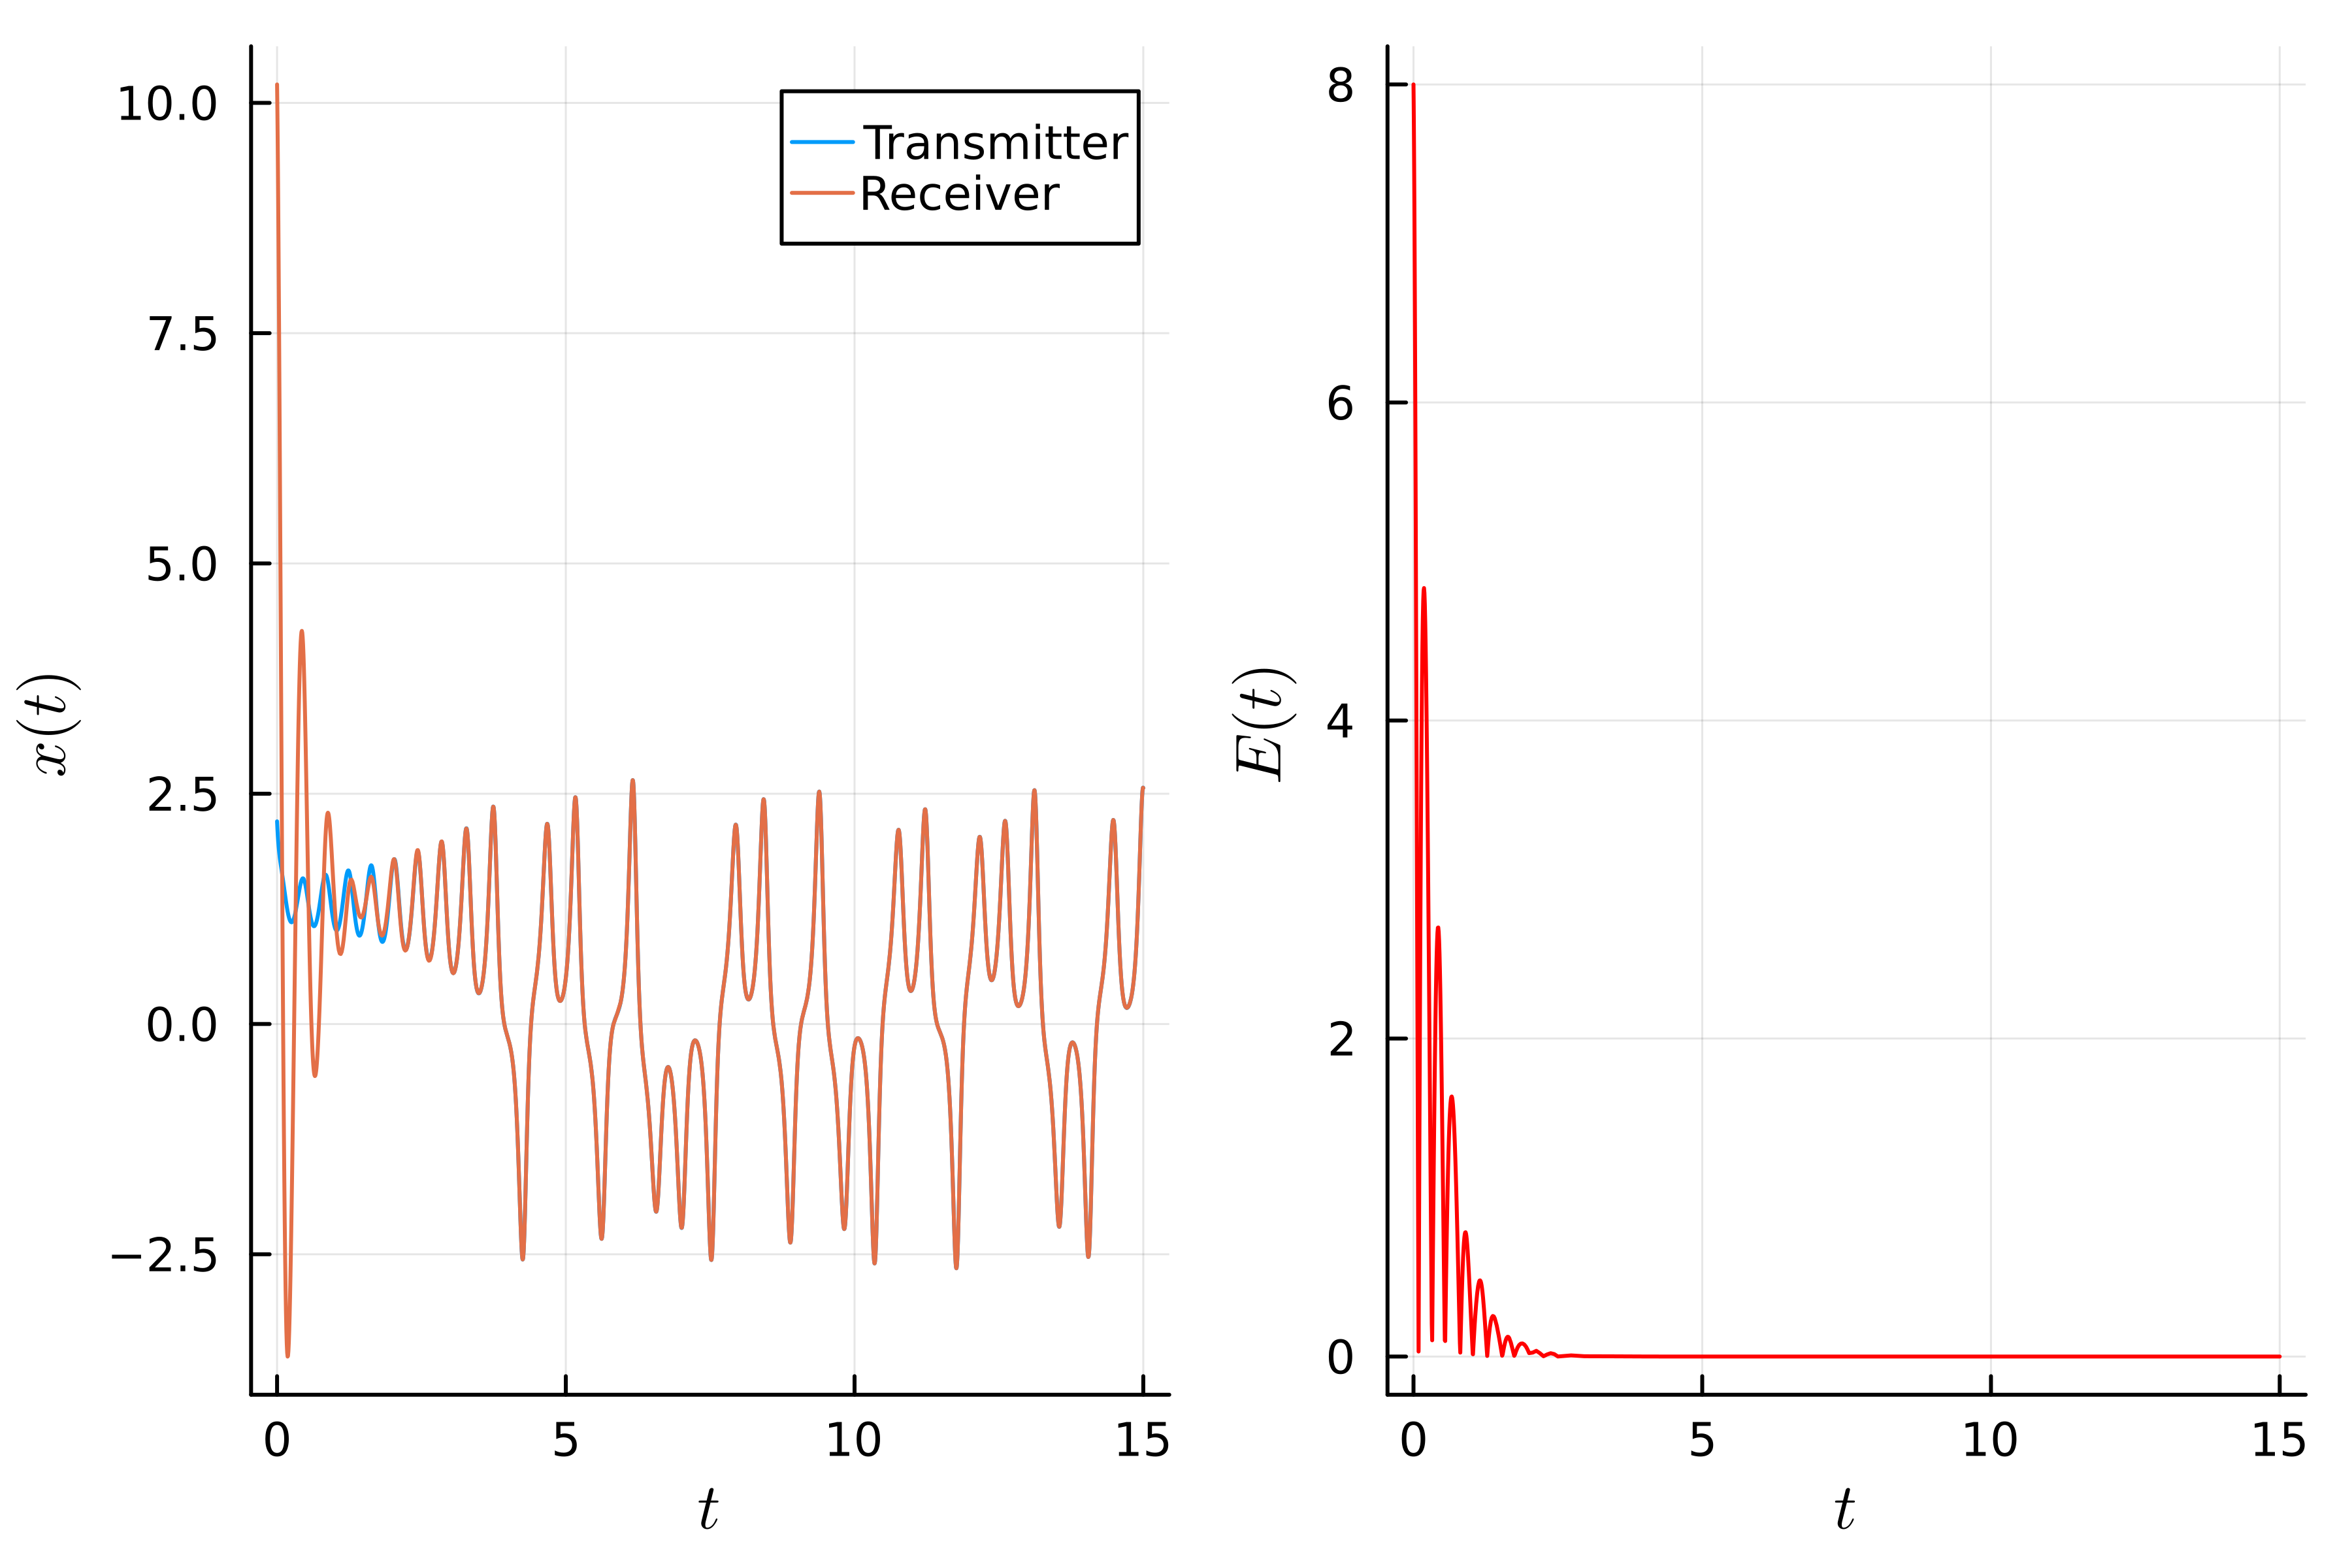
\includegraphics[width=\linewidth]{figures/combined_plot.png}
          \centering
          \caption{Plot of the $x$-component of both the transmitter and receiver's dynamical systems. The error $E(t) = |x_T - x_R|$ exponentially decrease to $0$.}
      \end{figure}
    \section{Applications to Communication and Numerical Experiments}
    We explore how synchronized chaotic systems can be used to encrypt messages. 
    \begin{figure}[H]
        
\includegraphics[width=8cm]{drawing.png}
        \centering
        \caption{The transmitter want to send a secret message $m(t)$ to the receiver and want no one else to be able to read it.}
    \end{figure}
    Consider two people: Transmitter and Receiver. Transmitter want to send a secret message $m(t)$ to Receiver. Cuomo and Oppenheim show that one way of solving this dilemma is by using synchronized chaotic system \cite{cuomo1993}. The core idea is to send the message $m(t)$ in the trajectory of the transmitter's dynamica system, use the receiver's dynamical system to reproduce the actual trajectory of the transmitter's dynamical system, and use this to directly compute $m(t)$. In their paper, they create a circuit implementation that capture the same behavior as the pair of dynamical systems. Compared to their paper, we will use the same algorithm by Cuomo and Oppenheim, but implement the algorithm numerically. 
    \subsection{Algorithm Implementation}
    Let $m(t)$ be the message the transmitter want to send to the receiver. The numerical algorithm is given below. 
    \begin{enumerate}
      \item Create encrypted message $\widetilde{m}(t) = x_T (t) + m(t)$ where $||m(t)|| \ll ||x_T(t)||$. 
        \item Send the encrypted message $\widetilde{m}(t)$ to the receiver. 
        \item Use the receiver's dynamical system to hopefully reproduce $x_R(t) \approx x_T(t)$. 
        \item Compute $\widetilde{m}(t) - x_R(t) \approx x_T (t) + m(t) - x_T(t) = m(t)$. 
    \end{enumerate}
    The first step is to create an encrypted message $\widetilde{m}(t) = x_T (t) + m(t)$ where the magnitude of $m(t)$ is much smaller than the magnitude of $x_T(t)$. This encrypt the message $m(t)$ because $x_T(t)$ serve as noise to hide the message $m(t)$. Note that $m(t)$ can be made as small as we like by multiplying by $\varepsilon > 0$. The receiver can multiply by $\frac{1}{\varepsilon}$ to get $m(t)$ back when the receiver recover the scaled version of $m(t)$.  

    The second step is to send the encrypted message $\widetilde{m}(t)$ to the receiver and the third step is to use $\widetilde{m}(t)$ to reproduce $x_T(t)$ before the trajectory got corrupted by noise. Note that in this case, $m(t)$ is noise as the receiver's dynamical system try to synchronize with $\widetilde{m}(t)$ which is corrupted by noise. The receiver's dynamical system is 
    \begin{equation*} 
      \begin{aligned}
        \dot{x_R} &= \sigma (y_R-x_R), \\
        \dot{y_R} &= r  \widetilde{m} - y_R - 20 (\widetilde{m}   z_R),\\
        \dot{z_R} &= 5 \widetilde{m} y_R - b  z_R,
      \end{aligned}
    \end{equation*}
    where $x_R$ is replaced by $\widetilde{m}$ except for the equation for $\dot{x_R}$. Also, notice that the receiver's dynamical system will not perfectly recover $x_T(t)$ because of the noise $m(t)$. 

    The last step is to compute the message $m(t)$ which is what the transmitter want to send. In step $3$, the receiver's dynamical systems hopefully reproduce $x_R(t) \approx x_T(t)$. Thus, $\widetilde{m}(t) - x_R(t) = (x_T(t) + m(t)) - x_T(t) = m(t)$. 

    In contrast to a circuit implementation of the algorithm, one concern is numerical errors. The tolerance of the differential equation solver should be set to sufficiently low values such that the digits representing $m(t)$ are not truncated or rounded in the solution. For this reason, we set the relative and absolute tolerance to $10^{-11}$. 

    % - numerical implementation of the algorithm and plots of convergence and noise and add pitfalls about machine epsilon 
    % - introduce it in the code format and mention particular findings that I found for this (numerical errors that can occur with rounding and what not)
    \subsection{Transmitting a Message}
    In order to transmit a message, we can convert an audio file to a waveform. For instance, the \verb|wav| library and \verb|Wav.jl| package are both capable of reading audio files and writing them into waveforms in Python and Julia respectively. Then, a linear interpolation can be done on the signal to create the message $m(t)$. After transmitting them to the receiver, the receiver can convert the waveforms into audio files to listen to them. 
    
    We use the transformation above to transmit the audio file \verb|taunt.wav|.\footnote{The audio file came from an introductory programming class taught at UIUC: \url{https://www2.cs.uic.edu/~i101/SoundFiles/}.} The parameters are the same as before which are $\sigma = 16$, $r=45.6$, and $b = 4$ and the intial conditions are the same for both systems which is $(2.2, 1.3, 2.0)$. The plot of the waveforms and error between the two waveforms are shown below. 
    \begin{figure}[H]
        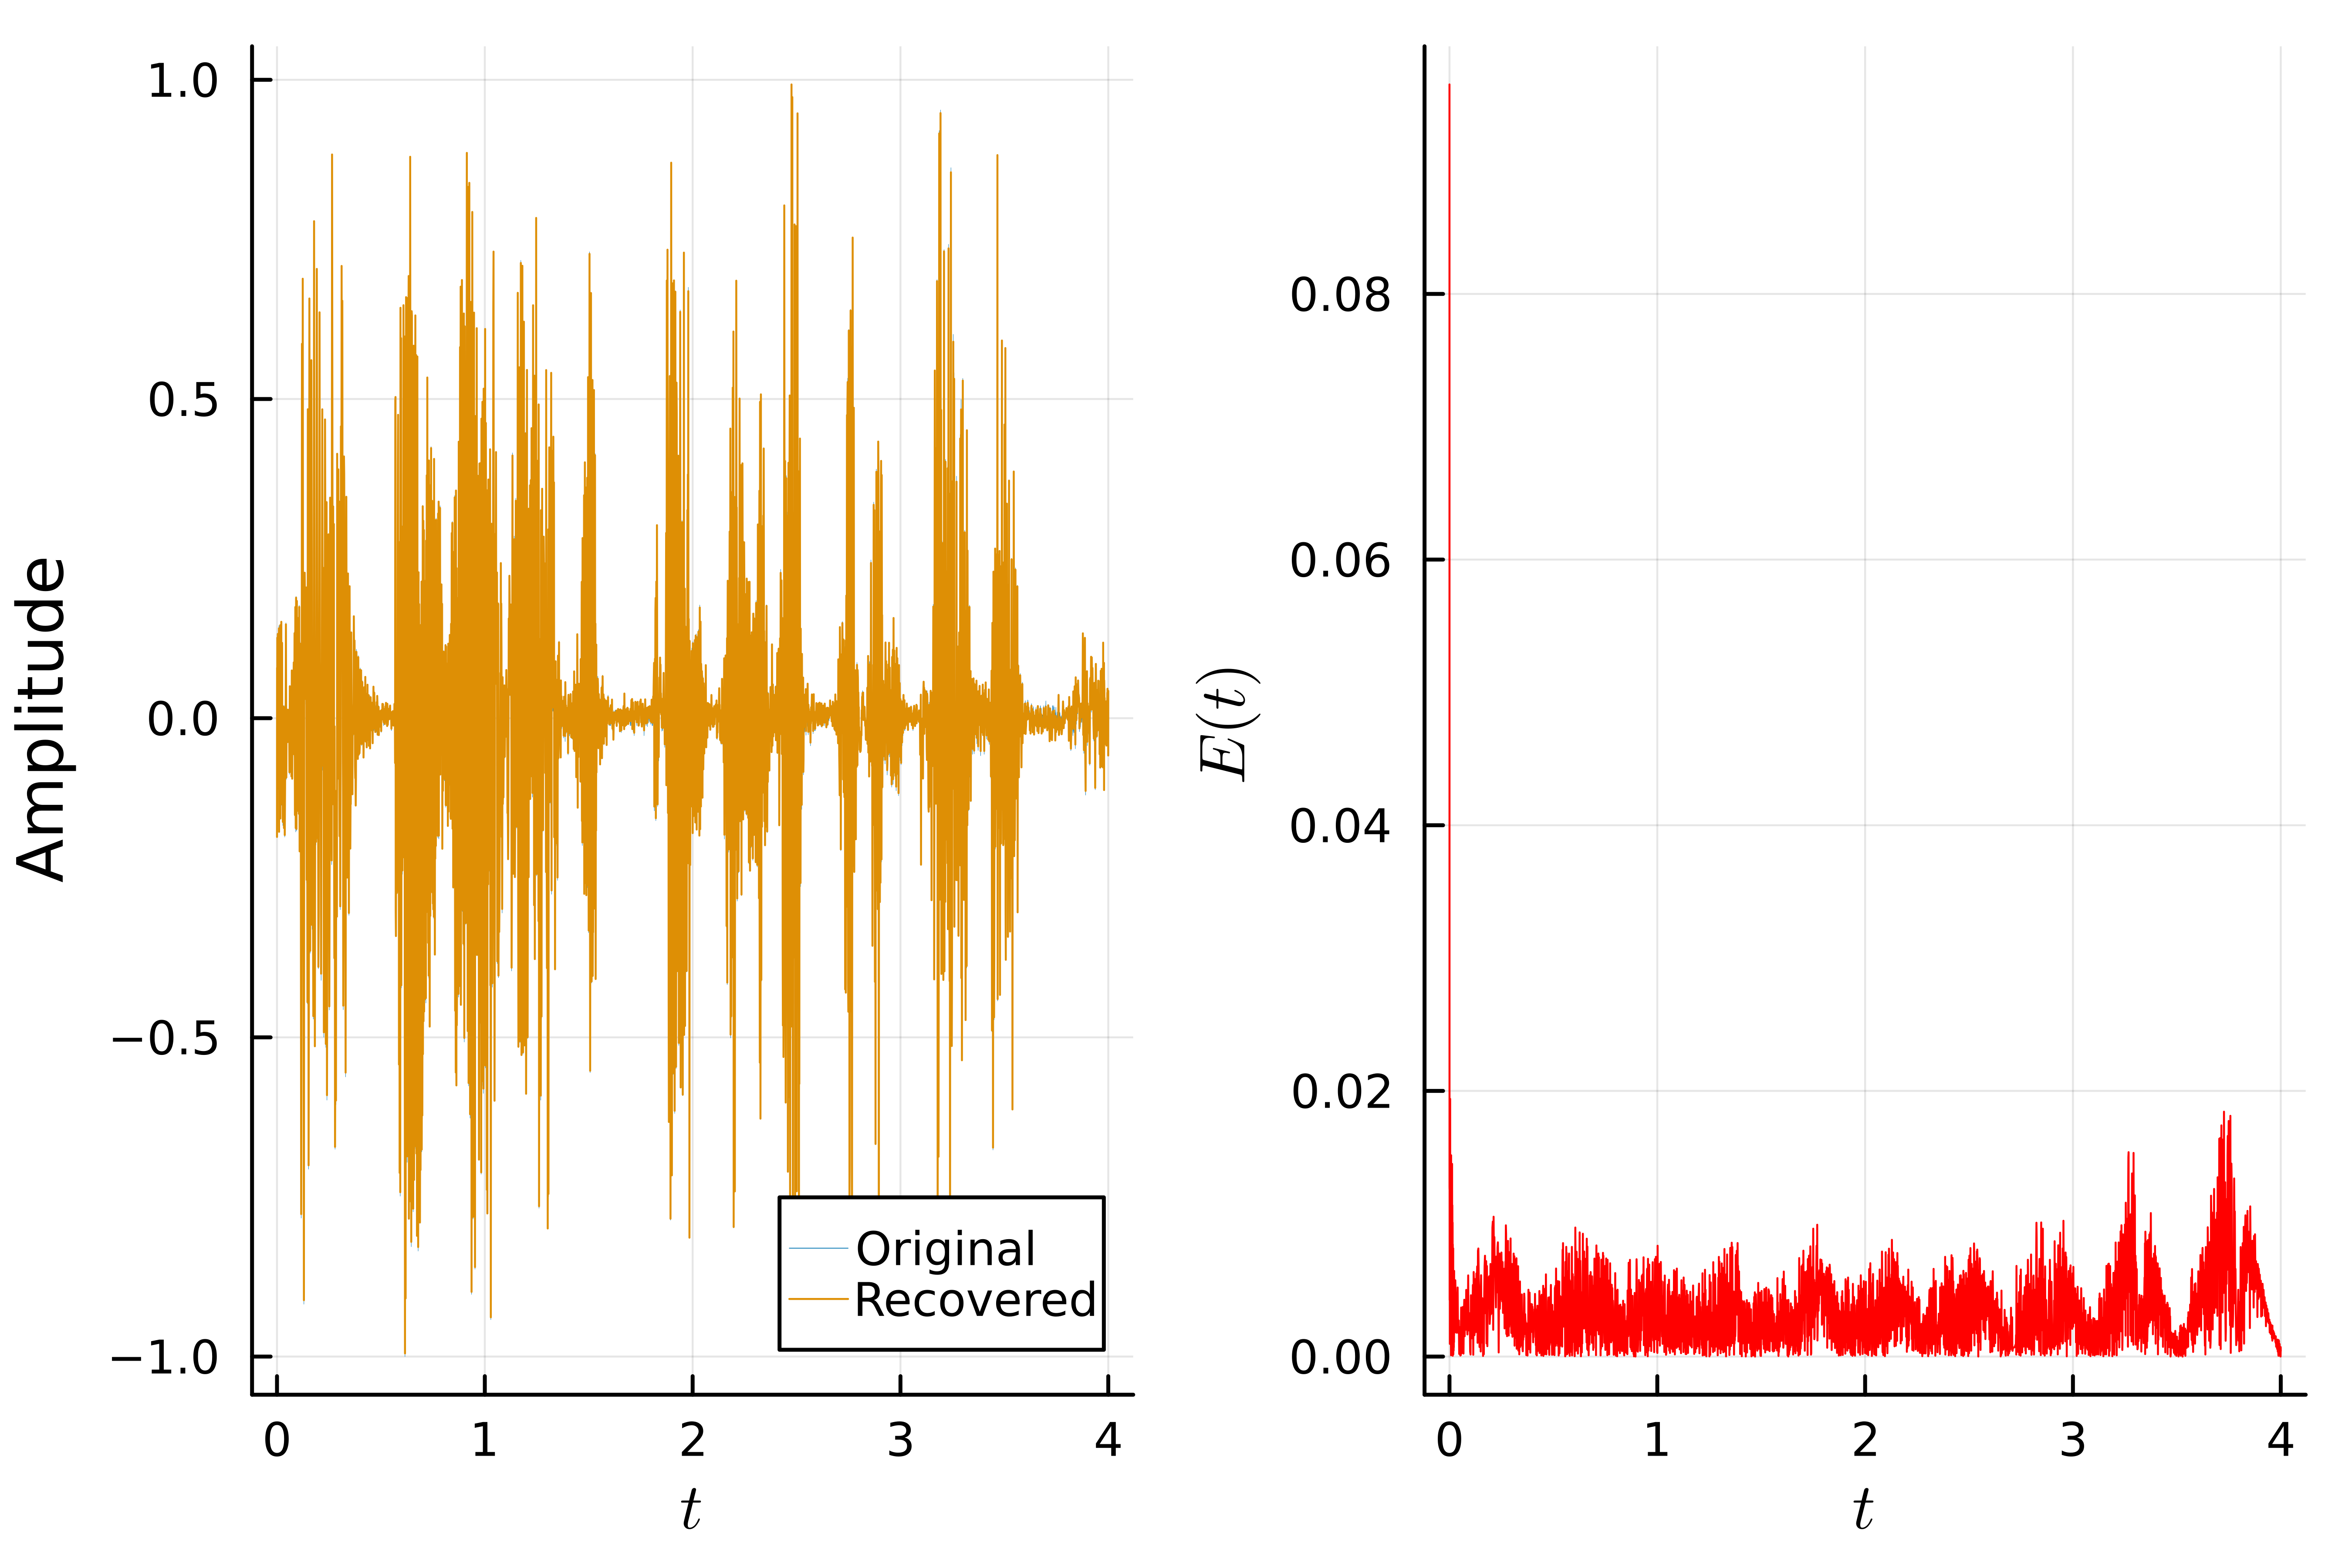
\includegraphics[width=\linewidth]{combined_error_sound_plot_paper.png}
        \centering
        \caption{Plot of both waveforms and the absolute error between the two waveforms.}
    \end{figure}
    Notice that the error is not completely zero due to the ``noise'' that is added due to $m(t)$. Despite this, the audio file produced from this is listenable and one can hear the message that is being sent. 
    \subsection{Testing Algorithm Against Noise}
    In non-idealized situations, there will always be noise that is transmitted along with the signal that we want to send. Similar to Cuomo, Oppenheim, and Strogatz, we also explore how Gaussian noise affect the quality of the recovered message \cite{chaoticnoise}. 

    Instead of sending the message $\tilde{m}(t) = x_T (t) + m(t)$, we send the message 
    \begin{equation*} 
      \tilde{m}(t) = x_T (t) + m(t) + N(0,\sigma^2)
    \end{equation*}
    where $N(0,\sigma^2)$ is Gaussian noise with variance $\sigma^2$. 

    We test it for various standard deviations $\sigma$: $0, 0.5, 1, 2$ and determine how well the algorithm withstand against noise by plotting the error between the original message and the recovered message. 
    \begin{figure}[H]
        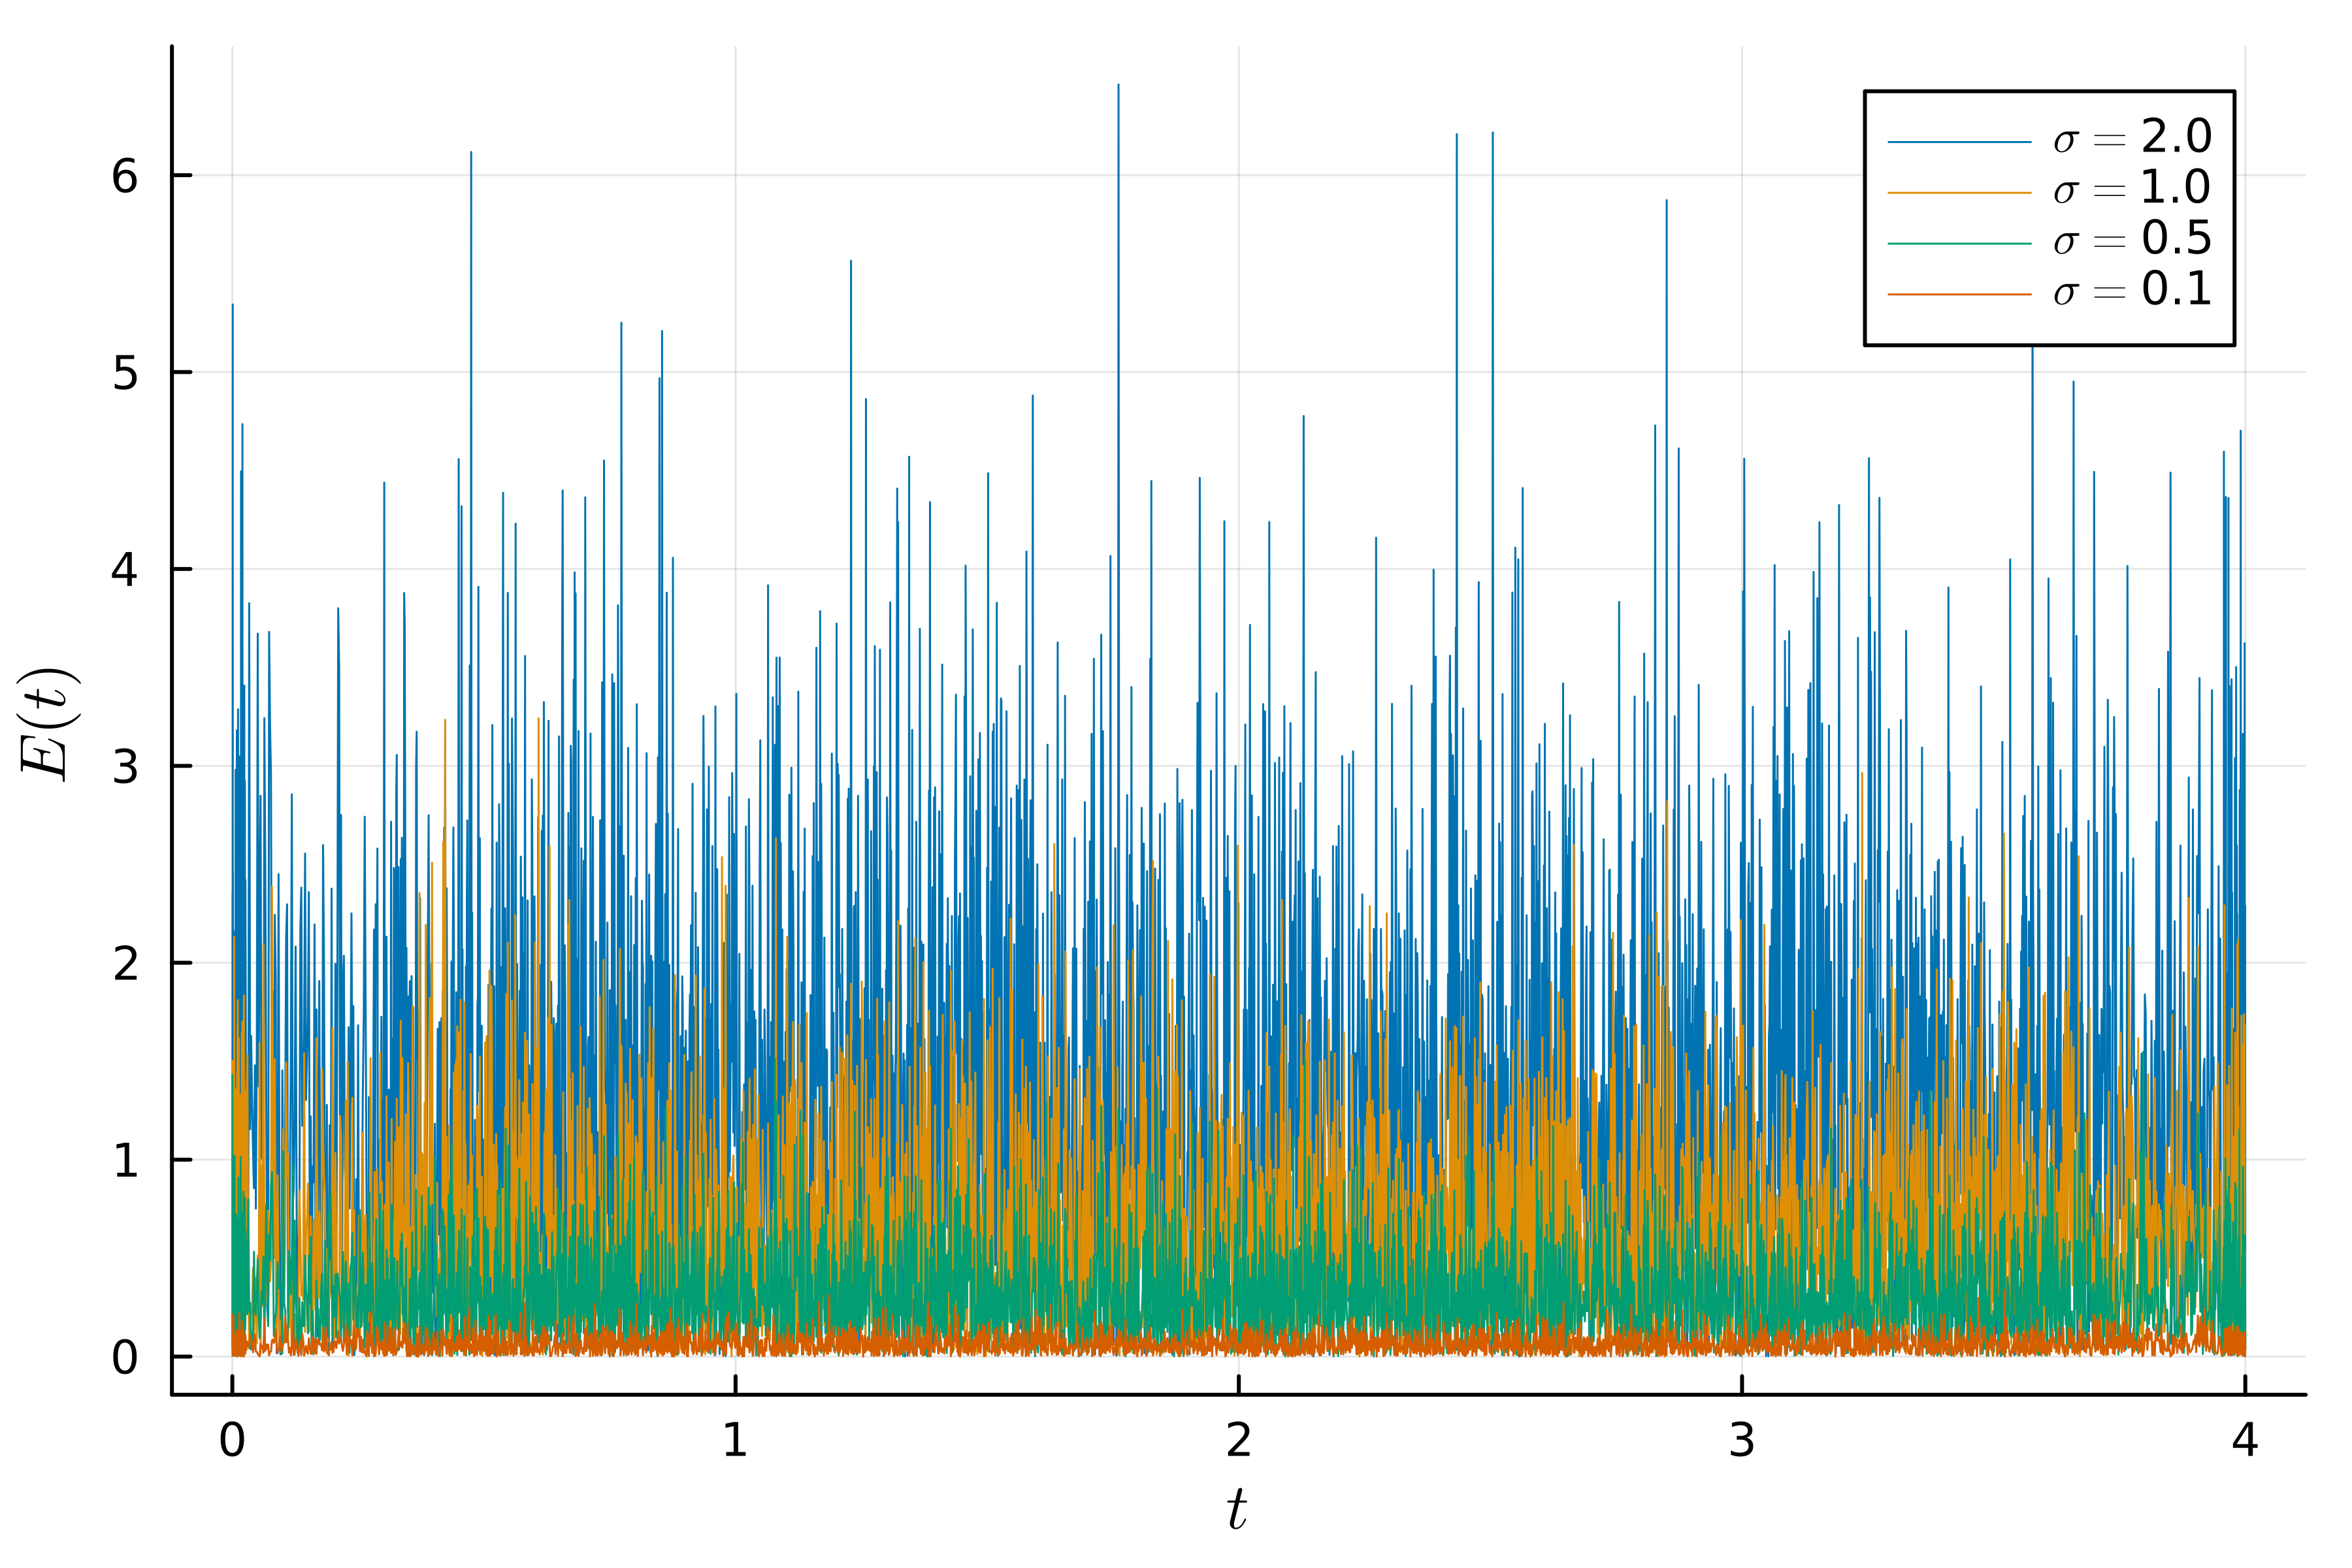
\includegraphics[width=\linewidth]{error_plot_noise.png}
        \centering
        \caption{A plot of the absolute error between the original message and the receovered message for various values of $\sigma$.}
    \end{figure}
    Recall that the magnitude of a waveform is $1$. As such, we might expect some distortion of the audio for $\sigma = 0.5$ or greater. However, the result was that the original message is remains, but the message is masked by static noise. For greater value of $\sigma$, the static noise eventually drown out the original message as in the case of $\sigma = 2$. This points that the algorithm is largely suspectible to noise and require a near perfect transmission of the encrypted message $\widetilde{m}(t)$ to recover the message $m(t)$. 


    \section{Conclusion}
    % - brief summary and future work 
  \newpage    
    \printbibliography
    \addcontentsline{toc}{section}{References}
\end{document}